%Autor: aplatanad, mojopikon
%aplatanad: 15 + 9
%mojopikon: 3

\chapter{El entorno X-Window}
\label{xwindow.tex}


\section{¿Qué es X-Window?}\index{X} 

En algunos  sistemas operativos  el entorno gráfico,  también conocido
como  {\em  GUI  (Graphic  User Interface)}\index{GUI}  es  una  parte
inherente al sistema.  En dichos casos los  diseñadores no concibieron
el funcionamiento de la máquina en situaciones donde el GUI sea inútil
o implique  un desperdicio innecesario  de recursos. En  esos sistemas
el  entorno  gráfico  no  sólo  no  suele  ser  sustituible  sino  que
sencillamente el sistema operativo no puede funcionar sin él. La mayor
parte  de los  sistemas operativos  que cumplen  esta descripción  son
sistemas jóvenes, desarrollados recientemente, con la clara convicción
de  que  el  entorno  gráfico  era  la  gran  panacea.  El  tiempo  ha
demostrado  que  estaban  parcialmente equivocados.  Disponer  de  GUI
facilita  el acceso  del gran  público  a la  informática, pero  resta
mucha flexibilidad  a los profesionales o  usuarios avanzados, cuyas
necesidades  siempre  van  un  paso  por  delante  de  las  soluciones
aportadas por el GUI. Prueba de ello es que algunos sistemas netamente
gráficos  han  comenzado a  cuidar  su  interfaz  de comandos  con  el
objetivo  de poder  introducirse en  el segmento  de los  servidores y
estaciones de trabajo profesionales.

La bases de los sistemas operativos UNIX actuales se establecieron por
Bell Laboratories en torno a 1970. En aquella época los ordenadores no
contaban con otra cosa que no  fuera una consola en modo texto. Dichos
sistemas  han evolucionado  a  lo largo  del  tiempo incorporando  las
correspondientes innovaciones  tecnológicas debidas a  la implantación
del modo  gráfico por  los ordenadores  de todo el  mundo. A  causa de
dicho  proceso  de evolución,  en  Linux  el  entorno gráfico  es  una
aplicación  más de  las muchas  que pueden  estar ejecutándose,  o no,
en  el  sistema. Por  lo  tanto  puede  ser sustituido  según  nuestra
conveniencia.

El entorno  gráfico más ampliamente  extendido en el  mundo UNIX/Linux
son las {\sf  X-Window}, conocidas comúnmente como  {\sf X}\index{X} a
secas.

\subsection{La arquitectura de las X} 

Las  {\sf   X}  presentan  una  arquitectura   (Figura  \ref{xwindow})
cliente/servidor que  en muchos  casos ha sido  alabada pero  en otros
muchos criticada.

\begin{figura}{xwindow}{1}
\caption{Arquitectura cliente/servidor del sistema X-Window}
\label{xwindow}
\end{figura}

La arquitectura de las {\sf X} se divide en dos elementos
fundamentales.  Por un lado el {\em servidor X}\index{servidor X}
encargado de gestionar el uso de los dispositivos de salida (p. ej.
tarjetas gráficas) y de los dispositivos de entrada (p. ej. teclados,
ratones, tabletas digitalizadoras, etc.) Por el otro lado, los {\em
clientes X}\index{cliente X} nombre con el que se conoce a cada una de
las aplicaciones que hacen uso del sistema {\sf X}. Las pulsaciones de
tecla, el movimiento del ratón o cualquier otra acción del usuario en
los dispositivos de entrada es detectada por servidor y transferida a
los clientes. De la misma manera los clientes transfieren al servidor
las peticiones de operaciones a realizar sobre el dispositivo de
salida (p. ej.  trazar un línea en pantalla, dibujar un punto, volcar
un bitmap, etc). La comunicación entre cliente y servidor sigue un
protocolo estandarizado que corre sobre los servicios de red del
sistema. Esto permite que los clientes no tengan por qué estar en la
misma máquina que el servidor. Eso quiere decir que podemos tener un
servidor {\sf X} en nuestra máquina local a través del que interactuar
con clientes que se ejecutan de forma remota en otro ordenador, sin
que por ello notemos diferencia alguna. Aparte de todo esto las {\sf
X} realizan ciertas optimizaciones en los casos en los que cliente y
servidor se encuentran en la misma máquina. Por ejemplo, se permite el
acceso directo al hardware de vídeo ignorando el protocolo descrito,
con lo que se aprovechan las características de aceleración 3D de
muchas tarjetas modernas. Con ello las {\sf X} se convierten en una
plataforma potente para ejecutar aplicaciones exigentes desde un punto
de vista gráfico sin por ello perder su flexibilidad.

Otra característica  interesante del  sistema {\sf  X} es  que podemos
tener varios  servidores en una  misma máquina,  donde cada uno  es un
{\em  ente}  independiente que  utiliza  sus  propios dispositivos  de
entrada y salida.  Evidentemente no es habitual disponer de  más de un
monitor o  teclado pero en  ocasiones se pueden  utilizar servidores
sin  salida gráfica.  También es  posible  que todos  usen los  mismos
dispositivos  y  que se  habilite  algún  mecanismo para  que  podamos
conmutar entre ellos a voluntad.

\subsection{Gestores de ventanas}

En  todo  buen  entorno  gráfico  moderno  las  aplicaciones  utilizan
ventanas para interactuar con el usuario. Sin embargo el servidor {\sf
X}  sólo entiende  un  número limitado  de  primitivas gráficas,  como
dibujar  líneas y  puntos  o copiar  áreas de  la  pantalla. Por  ello
se  hace  necesaria  la  presencia  de  una  aplicación  cliente  {\em
especial}  que se  encargue de  crear, destruir,  mover, gestionar  el
foco  y  en  general  gestionar todas  las  cuestiones  referentes  al
comportamiento de  las ventanas,  utilizando para ello  las primitivas
del servidor  {\sf X}. A dicha  aplicación se la denomina  {\em gestor
de  ventanas}\index{gestor de  ventanas}. En  la Figura  \ref{xwindow}
podemos  ver  su situación  dentro  de  la  arquitectura de  las  {\sf
X-Window}.

En una  distribución de  Linux puede  haber cerca  de  40  gestores de
ventanas  entre los  que un  usuario debe  elegir. Cada  uno de  ellos
imprime  un {\em  feeling}  o  sabor diferente  a  nuestro entorno  de
trabajo. Tengamos en  cuenta que cada gestor dibuja  los elementos del
marco  de nuestras  ventanas  de  forma diferente  (e.j.  la barra  de
título,  los  botones  de  control,  los  bordes),  dotándolos  de  un
comportamiento particular y característico  según las preferencias del
equipo de programadores que lo diseñó. Empezando por los estéticamente
más valorados como  {\sf Window Maker} o  {\sf Enlightenment}; pasando
por los que  imitan a otros sistemas como {\sf  AfterStep} o {\sf F(?)
Virtual Window  Manager} (en una  de sus variantes nos  proporciona el
look de Microsoft® Windows® 95); o los que permiten ser personalizados
con  {\em temas}  diferentes  como  {\sf Ice  Window  Manager} o  {\sf
Sawfish}; y  terminando por los  más ligeros  y rápidos pero  no menos
funcionales como  {\sf Fast  Light Window Manager}  se cubre  toda una
variedad de necesidades del usuario.

\subsection{Entornos de escritorio}

Ahora que  disponemos de  ventanas se  hace necesario  rellenarlas con
algo. A la hora de programar una  aplicación para las {\sf X} se suele
recurrir a  los {\em toolkits}\index{toolkits}. Se  trata de librerías
diseñadas  para proporcionar  diferentes  tipos de  controles (p.  ej.
botones,  barras de  menús, cuadros  de edición,  etc) facilitando  su
gestión. Las toolkits  crean los controles allí dónde  le digamos, los
destruyen,  los  redibujan  cuando  es necesario,  manejan  todas  las
acciones que se  hagan sobre ellos a  través del uso de  alguno de los
dispositivos de entrada  posibles, etc. Trabajar sin hacer  uso de los
toolkits implicaría diseñar y gestionar nuestros propios controles.

Es importante  destacar que una  aplicación {\sf X} funciona  sea cual
sea el  gestor de ventanas  seleccionado. Por tanto,  el uso de  uno u
otro es  una elección  personal del  usuario. Sin  embargo, el  uso de
un  toolkit  u otro  en  una  aplicación  es  elección del  equipo  de
programadores que ha  trabajado en ella. Eso unido a  la gran variedad
de toolkits  existente en  Linux convierte  nuestro escritorio  en una
selva  donde podemos  ver  una fauna  de  aplicaciones con  interfaces
gráficas de lo más variopinto.

Para garantizar  que las aplicaciones presenten  una interfaz similar,
reduciendo la curva de aprendizaje  de los usuarios, han aparecido los
{\em entornos de  escritorio}. Básicamente se trata  de establecer una
serie de  reglas comunes  que suelen incluir:  el toolkit  a utilizar,
el  formato  de la  ayuda,  el  modelo  de componentes,  librerías  de
tratamiento de  imágenes y sonido, etc.  Todo ello genera un  marco de
trabajo  tanto  para los  desarrolladores  de  nuevas como  de  viejas
aplicaciones.  Si  los  desarrolladores  se ciñen  a  dicho  marco  el
resultado es un entorno de trabajo  uniforme y cómodo donde no existen
diferencias sustanciales en la interfaz de una aplicación a otra.

Afortunadamente  la variedad  es una  característica de  Linux. En  la
actualidad disponemos de dos grandes entornos de escritorio:

\begin{description}

\item[GNOME]\index{GNOME} Funciona con el toolkit {\sf GTK}\index{GTK}
que fue originalmente diseñado para {\sf GIMP}. Quizás las principales
ventajas de este entorno no estén  tanto del lado del usuario como del
de los programadores, de la  tecnología que subyace debajo del sistema
y de la declaración de intenciones con la que se inició el proyecto.

\item[KDE]\index{KDE} Funciona sobre el toolkit {\sf Qt}\index{Qt}, lo
cual provocó una  gran polémica en sus orígenes al  no disponer de una
licencia todo  lo {\em libre}  que se  deseaba. En la  actualidad esos
problemas se  han resuelto y es,  hoy por hoy, considerado  por muchos
como el entorno con la interfaz más atractiva de los dos.

\end{description}

Cada  uno tiene  sus más  y sus  menos pero  la gran  realidad es  que
presentan una interfaz muy intuitiva que se aprende a manejar desde el
primer momento.

\section{Trabajar con las X-Window}

Al iniciar  un sistema Linux  con las  {\sf X} instaladas  es probable
que  se  nos  permita  autentificarnos   desde  el  modo  gráfico.  En
caso  contrario  sólo dispondremos  de  una  consola esperando  a  que
introduzcamos el  nombre de  usuario. Si nuestro  caso es  este último
debemos  autentificarnos, y  ejecutar el  comando {\tt  startx} cuando
el  sistema nos  indique  que está  disponible  para recibir  nuestros
comandos.  El  comando  {\tt  startx}  iniciará  el  entorno  gráfico.
Evidentemente al terminar nuestro trabajo volveremos a la consola.

\begin{figura}{gdm}{0.98}
\caption{Ventana de autentificación de GDM}\label{gdm}
\end{figura}

Para  que la  autentificación desde  el  modo gráfico  sea posible  es
necesario  tener  instalado  un  {\em  display  manager}\index{Display
manager}.    Algunos   de    ellos    son   {\tt    xdm}\index{Display
manager!xdm}, {\tt  kdm}\index{Display manager!kdm} ({\sf  KDE}), {\tt
gdm}\index{Display  manager!gdm}  ({\sf  GNOME}), etc.  En  la  Figura
\ref{gdm} podemos ver un ejemplo de la clásica ventana que nos muestra
{\sf GDM} nada más terminar la carga del sistema. Básicamente nos está
pidiendo nuestro nombre  de usuario, para una vez  pulsado {\tt Enter}
pedirnos la contraseña. Con  esa información seremos autentificados en
el  sistema y  se  iniciará una  nueva sesión  con  nuestra cuenta  de
usuario. Es importante  destacar que dentro de nuestra  sesión todo lo
que hagamos  es personal. Eso quiere  decir que los cambios,  sean del
tipo que sean, sólo afectarán a nuestra sesiones futuras pero no a las
de los otros usuarios de la máquina.

Antes  de continuar  es importante  destacar algunas  cosas. En  Linux
existe lo que se  denomina {\em terminales virtuales}\index{terminal}.
Si estamos  en modo texto podemos  usar la combinación de  teclas {\tt
A-F*} para  pasar de un terminal  a otro. Eso se  comprueba fácilmente
porque vemos  cómo cambia el contenido  de la pantalla. El  uso de los
terminales virtuales  nos permite mantener varias  sesiones abiertas y
trabajar de forma independiente en ellas. Cuando se inicia un servidor
{\sf  X} éste,  queda  asociado  a uno  de  esos terminales  virtuales
(podemos tener  varios servidores  asociados a  distintos terminales);
normalmente al  {\tt F7}. Debido al  mecanismo por el que  las {\sf X}
manejan el teclado,  en los terminales asociados a  servidores {\sf X}
ya  no se  puede usar  {\tt A-F*}  sino que  para cambiar  de terminal
debemos usar {\tt C-A-F*}. Usando  la primera combinación de teclas en
los terminales en modo texto, y la  última en los asociados a las {\sf
X}, no  tendremos problemas para  movernos por  ellos y pasar  de modo
gráfico a consola a nuestro antojo.

\begin{figura}{terminales}{0.98}
\caption{Diagrama de cómo se pasa de una terminal a otra.}
\label{terminales}
\end{figura}

Otro punto  importante es que sólo  cuando veamos un mensaje  del tipo
{\tt Kernel Panic}  podemos decir que nuestro Linux se  ha colgado. En
cualquier  otro  caso  estamos  frente a  sencillos  cuelgues  de  las
aplicaciones con  las que  trabajamos. No debemos  preocuparnos puesto
que Linux proporciona  los suficientes recursos como  para que podamos
recuperar el control de la máquina.  Por ejemplo, podemos cambiar a un
terminal diferente  de la consola  para matar aplicaciones que  se han
quedado colgadas en nuestro terminal de trabajo  o en las {\sf X} . En
situaciones críticas puede  ser necesario terminar con las  {\sf X} de
forma prematura. Para  ello se pulsa la  secuencia {\tt C-A-Backspace}
que  cierra  el servidor  {\sf  X}  abortando todas  las  aplicaciones
gráficas. Evidentemente los datos no guardados se perderán.

En Linux, cuando queremos ejecutar aplicaciones de modo consola dentro
de una ventana {\sf X} se utilizan los {\em emuladores de terminal}.
El más básico es el {\tt xterm}\index{xterm} que viene con la
instalación estándar de las {\sf X}, pero existen muchos otros y cada
entorno suele venir con uno propio. El de {\sf GNOME} está en {\tt
MENÚ PRINCIPAL $\rightarrow$ SISTEMA $\rightarrow$ TERMINAL UNIX DE
GNOME}, mientras que al de {\sf KDE} podemos acceder pulsando en el
icono con un terminal y una concha disponible en el panel de dicho
entorno de escritorio (Figura \ref{kde_panel}).  En ocasiones es
posible que intentemos ejecutar una aplicación que nunca llega a
mostrar su ventana principal o que da algún tipo de error grave. En
esos casos es recomendable ejecutar el programa desde un emulador de
terminal. Como ya hemos comentado, las aplicaciones para {\sf X} no
son diferentes de otras, por lo que suelen mostrar información por la
consola, si esta está disponible.  Esa información puede ser vital
para resolver nuestro problema.

Cuando ejecutamos una aplicación {\sf X} desde el emulador de terminal
(p. ej. {\tt xclock}) vemos que éste se queda bloqueado a la espera de
que la aplicación termine. Esto no debería sorprendernos puesto que en
realidad ocurre lo mismo cuando  ejecutamos una aplicación de consola.
Para que eso no suceda debemos añadir un {\tt \&} al final del comando
de la  aplicación {\sf X},  o pulsar {\tt  C-Z} y ejecutar  el comando
{\tt bg}\index{bg} sobre el emulador después de que la aplicación haya
sido iniciada. De esta manera la  aplicación {\sf X} pasa a ejecutarse
en segundo  plano, liberando  al emulador de  terminal para  que pueda
recibir nuevos comandos.

En  general mostrar  el  clásico  aviso de  que  una aplicación  tiene
archivos  modificados y  va a  ser  cerrada es  responsabilidad de  la
propia aplicación. El cierre de  la ventana principal por la pulsación
del  correspondiente botón  en la  barra  de título  es notificado  al
proceso propietario de la ventana.  Normalmente se suele mostrar dicho
mensaje  y una  vez aceptado  se termina  el proceso.  Sin embargo  es
posible que nuestra aplicación no  disponga de esa característica. Por
ejemplo, si cerramos  el emulador de terminal (muy pocos  avisan de la
posible pérdida de datos) cuando estamos ejecutando sobre él cualquier
tipo de  aplicación (sea  de consola  o de  {\sf X})  dicha aplicación
termina  inmediatamente perdiéndose  los  datos que  no hubieran  sido
guardados. O sea,  si ejecutamos {\tt gnome-edit} o  {\tt kedit} sobre
el terminal,  escribimos algo  en el editor,  y cerramos  el terminal,
veremos como nuestra aplicación de edición terminará sin advertir nada
de la pérdida de datos, y el terminal se cerrará sin indicarnos que se
encuentra esperando por el editor.

\begin{figura}{btitulo}{0.6}
\caption{Barra de título del gestor de ventanas Sawfish}\label{btitulo}
\end{figura}

Por otro lado es posible que el  proceso esté bloqueado y no reciba el
mensaje. En ese caso la ventana no  se cerrará a menos que forcemos su
destrucción con la  opción correspondiente en el menú del  marco de la
venta  (Figura  \ref{btitulo}, botón  de  la  izquierda). Entonces  el
gestor de ventanas la cerrará  pero la aplicación seguirá ejecutándose
en segundo plano aunque para nosotros  ya no exista. La única solución
será matarla  a mano  con el comando  {\tt kill}\index{kill}  desde un
emulador de terminal. Si vemos un consumo de CPU excesivo o un sistema
demasiado lento puede  deberse a la existencia de  procesos en segundo
plano que no fueron destruidos en su momento.

Una  aplicación   interesante  es  {\tt  xkill}\index{xkill}.   Si  la
ejecutamos nos  aparecerá un  punto de  mira en  el cursor  de nuestro
ratón.  Al  pulsar sobre  una  ventana  la  aplicación se  encarga  de
destruir al  proceso asociado  a la misma.  La aplicación  {\tt xkill}
puede ser lanzada desde un emulador de terminal o desde los cuadros de
diálogo de  las opciones {\tt  LANZAR} o  {\tt EJECUTAR} de  los menús
principales de los distintos entornos de escritorio.

Como hemos dicho anteriormente, a la  hora de aprender a usar las {\sf
X} no basta  con jugar con los botones izquierdo  y derecho de nuestro
ratón. En  las {\sf X}  el botón central  es de tanta  importancia que
suele disponer de funciones adicionales  que no están presentes en los
otros dos. En entornos de escritorio como {\sf KDE} o {\sf GNOME} esto
suele implicar un menú de contexto  adicional al que se muestra usando
el botón derecho; pero en  otras aplicaciones podemos encontrar formas
de manejo de lo más curiosas. Tal  es su importancia que en caso de no
disponer de él se emula por la pulsación simultanea de los dos botones
estándar del ratón. Una aplicación interesante del botón central es su
uso para copiar texto entre aplicaciones, sea cual sea la toolkit bajo
las que hayan sido desarrolladas. Basta con marcar nuestro texto en la
aplicación de  origen para  que al  pulsar el botón  central en  la de
destino éste se pegue a continuación de la posición actual del cursor.
En el  servidor {\sf  X} existe un  búffer que se  llena cada  vez que
marcamos texto  en alguna  aplicación. El botón  central del  ratón lo
único que hace es volcar ese  texto como si hubiera sido escrito desde
el teclado. Por tanto para utilizar  este sistema es importante ser lo
suficientemente cuidadoso  como para  no marcar  otra cosa  después de
marcar el texto a copiar.

\section{El escritorio de GNOME}\index{GNOME}

Debido a la sencillez de los  entornos de escritorio resulta 
inútil intentar explicar  detalladamente su manejo. La  mejor forma de
aprender es  sentarnos delante de uno  de ellos, ser un  poco osado, y
ante todo tener la buena  costumbre de leer detenidamente todo aquello
que nos indique el sistema. Sin  embargo, vamos a realizar una primera
toma  de contacto  guiada  en la  que  aprenderemos algunos  conceptos
básicos que  nos serán de  gran ayuda en  el futuro. Para  empezar nos
centraremos  en  uno de  los  dos  entornos  de escritorio  que  hemos
comentado anteriormente. Concretamente echaremos un vistazo al entorno
de escritorio  {\sf GNOME}\index{GNOME}.  Sin embargo, los  devotos de
{\sf  KDE} no  deben  preocuparse puesto  que  conociendo uno  resulta
extremadamente sencillo  llegar a dominar  el otro. Aun así,  al final
del  capitulo,  comentaremos  algunos  aspectos de  interés  sobre  el
fantástico entorno de escritorio de {\sf KDE}.

\subsection{GNOME Display Manager}
\index{GNOME!Display Manager,GNOME!gdm,Display manager!gdm}

Si  nuestro sistema  tiene  instalado el  entorno  de escritorio  {\sf
GNOME} y permite la autentificación  desde el modo gráfico es probable
que tengamos instalado el {\sf  GDM (GNOME Display Manager)} como {\em
display  manager}(Figura  \ref{gdm}).  {\sf GDM}  dispone  de  algunas
opciones adicionales que  podemos emplear antes de  iniciar el proceso
de autentificación,  y que no  tienen porque estar presentes  en otros
display manager.

\begin{description}

\item[SESIÓN] Nos permite elegir la  naturaleza de la próxima sesión a
iniciar. Opciones habituales son {\sf GNOME} y {\sf KDE}. Eligiéndolas
iniciaremos  sesión  con  el  entorno de  escritorio  que  prefiramos.
También puede haber alguna sesión especial {\em a prueba de fallos}, o
que carezca de  un entorno de escritorio específico,  o cualquier otro
tipo de sesión que el  administrador del sistema haya deseado incluir.
La opción por defecto es {\tt ÚLTIMA} que hace referencia a entrar con
el tipo de sesión que tenemos  asignado nosotros por defecto. Si nunca
hemos elegido  ninguno lo normal es  que el tipo por  defecto sea {\sf
GNOME}. Si hacemos una selección diferente  a la opción por defecto el
sistema nos  preguntara si queremos  que el  nuevo tipo de  sesión sea
nuestra sesión por defecto, y por  tanto a la que que corresponderá la
opción {\tt ÚLTIMA} la próxima vez.

\item[IDIOMA] Aparte  de elegir  sesión podemos seleccionar  el idioma
con el  que queremos  trabajar. Las aplicaciones  traducidas mostrarán
toda la información  en dicho idioma. Igual que antes,  la opción {\tt
ÚLTIMA}  habla de  nuestra última  selección, es  decir el  idioma por
defecto.

\item[SISTEMA] Nos  permite apagar, suspender o  reiniciar la máquina.
En algunos sistemas,  y siempre y cuando dispongamos  de la contraseña
de la  cuenta del  {\tt root},  nos permite  configurar {\sf  GDM}. Es
importante recordar que al cerrar nuestra sesión volvemos a la ventana
de {\sf GDM}  por lo que si  deseamos apagar el sistema  éste sería el
momento de seleccionar la opción correspondiente.

\end{description}

\subsection{Paneles y menús de GNOME}

Suponiendo  que iniciamos  sesión en  la  máquina lo  primero que  nos
llamará la atención son los  {\em paneles} (Figuras \ref{gnome_menu} y
\ref{gnome_menu_principal}).  

\begin{figura}{gnome_menu}{0.98}
\caption{Menú de panel de {\sf GNOME}}\label{gnome_menu}
\end{figura}

Si  pulsamos  en  la  huella   del  panel  inferior,  o  seleccionamos
alguna  de las  opciones del  panel superior,  dispondremos de  acceso
a  las  aplicaciones instaladas  en  el  sistema.  La mayor  parte  de
las  aplicaciones  {\sf GNOME}  están  clasificadas  y disponibles  en
alguno de  los submenús correspondientes. (p.  ej. {\tt APLICACIONES},
{\tt  UTILIDADES},  {\tt  GRÁFICOS},  etc).  En  {\tt  MENÚS  KDE}  se
encuentran clasificadas todas las aplicaciones {\sf KDE} instaladas, y
en  {\tt MENÚS  DEBIAN}  todas las  aplicaciones  de la  distribución,
independientemente  del  entorno de  escritorio  para  las que  fueron
desarrolladas.  En  este  punto  es importante  recordar  que  podemos
ejecutar  cualquiera  de las  aplicaciones  sin  importar que  estemos
trabajando en un  entorno de escritorio diferente a aquel  para el que
fueron diseñadas.

\begin{figura}{gnome_menu_principal}{0.55}
\caption{Panel alineado de {\sf GNOME} y menú principal}
\label{gnome_menu_principal}
\end{figura}

Otras opciones son el menú  {\tt FAVORITOS}, que es personalizable con
nuestras aplicaciones preferidas usando la opción {\tt AÑADIR DESDE EL
MENÚ}  (Figura  \ref{gnome_favoritos}),  la opción  {\tt  BLOQUEAR  LA
PANTALLA}, para proteger nuestro escritorio si tenemos que abandonarlo
por  cualquier  motivo  (es  importante recordar  que  de  esa  manera
evitaremos  que  manipulen  nuestros   datos  pero  siempre  queda  la
posibilidad de que  pulsen {\tt C-A-Backspace} para  abortar todas las
aplicaciones gráficas, perdiendo los datos  no guardados y volviendo a
la  ventana de  inicio de  sesión  del {\sf  GDM}), y  la opción  {\tt
TERMINAR SESIÓN}  para terminar nuestra  sesión y volver al  {\sf GDM}
(Figura \ref{gdm}).

\begin{figura}{gnome_favoritos}{0.98}
\caption{Añadir elemento al menú {\tt FAVORITOS}}
\label{gnome_favoritos}
\end{figura}

En  {\sf  GTK},   y  por  tanto  en  {\sf  GNOME},   todos  los  menús
cuentan  con   una  pequeña  marca   en  la  parte   superior  (Figura
\ref{gnome_menu_persis}). Si pulsamos en ella  el menú se desprende de
la aplicación  y pasa  a estar  en una  ventana independiente.  De esa
manera podemos acceder a un menú con opciones de uso habitual de forma
más rápida y sencilla.

\begin{figura}{gnome_menu_persis}{0.98}
\caption{Hacer que un menú sea persistente}
\label{gnome_menu_persis}
\end{figura}

Tal y  como podemos  apreciar en la  Figura \ref{gnome_menu_contexto},
todos los elementos del menú principal disponen de un menú de contexto
que se despliega cuando pulsamos con el botón derecho de nuestro ratón.
Entre las  opciones de  dicho menú contamos  con algunas  que permiten
añadir el elemento al panel,  quitarlo del menú principal, añadirlo al
menú {\tt  FAVORITOS} o  alterar sus  propiedades, entre  muchas otras
alternativas.

\begin{figura}{gnome_menu_contexto}{0.6}
\caption{Menú de contexto de los elementos del menú principal}
\label{gnome_menu_contexto}
\end{figura}

Una de las  opciones más interesantes de dicho menú  de contexto es la
que  se encuentra  bajo el  texto de  {\tt PONER  EN EL  FORMULARIO DE
EJECUCIÓN}. Esa opción abre el cuadro de diálogo {\tt LANZAR PROGRAMA}
y lo rellena con las propiedades del elemento del menú principal sobre
el que estamos trabajando. Ese  mismo cuadro está disponible como {\tt
LANZAR} en el menú principal. En la Figura \ref{gnome_lanzar} vemos el
cuadro  de diálogo  {\tt LANZAR  PROGRAMA}, que  podremos observar  si
seleccionamos  dicha  opción.  En  dicho  cuadro  de  diálogo  podemos
seleccionar la aplicación {\sf GNOME}  que deseamos ejecutar, así como
añadirla al menú  de favoritos. El mismo cuadro de  diálogo dispone de
{\em  opciones  avanzadas}  (Figura  \ref{gnome_lanzar_avd})  que  nos
permiten especificar la línea de comandos a ejecutar o especificar que
deseamos  que  la aplicación  se  ejecute  dentro  de un  emulador  de
terminal. La primera de las opciones resulta especialmente interesante
si la aplicación  no está disponible entre las que  nos permite elegir
el cuadro  de diálogo (p. ej.  {\tt xkill}) o porque  queramos pasarle
alguna opción de la línea de comandos de la aplicación.

\begin{figure}[hbtp]
\centering
\subfigure[Cuadro de diálogo {\tt LANZAR PROGRAMA}]{%
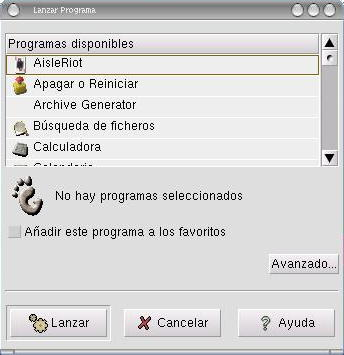
\includegraphics[width=0.45\textwidth]{imagenes/gnome_lanzar.eps}
\label{gnome_lanzar}}
\subfigure[Cuadro de diálogo avanzado {\tt LANZAR PROGRAMA}]{%
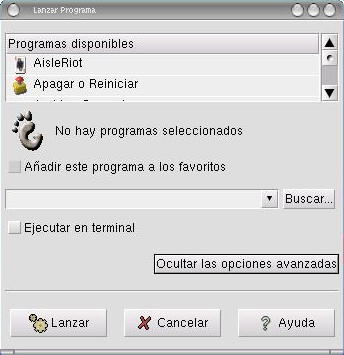
\includegraphics[width=0.45\textwidth]{imagenes/gnome_lanzar_avd.eps}
\label{gnome_lanzar_avd}}
\end{figure}

Manejar  {\sf  GNOME} es  cuestión  de  jugar  un  rato y  probar  las
diferentes opciones. Disponemos  de tres botones en  nuestro ratón (ya
hablamos de  eso en  apartados anteriores) y  se trata  de utilizarlos
sobre los elementos del entorno para ver como reaccionan. Por ejemplo,
si pulsamos  con el botón derecho  del nuestro ratón sobre  algún área
sin elementos de  algunos de los paneles, veremos un  menú de contexto
similar  al menú  principal del  que  hemos estado  hablando hasta  el
momento.  En el  menú  del  que estamos  hablando  existe un  elemento
denominado {\tt PANEL} que contiene  las opciones de configuración del
panel. Con dichas opciones podemos:

\begin{description}

\item[AÑADIR AL PANEL] Esta opción nos permite añadir nuevos elementos
al  panel.  A  parte  de  los  tipos de  botones  entre  los  que  nos
deja  elegir,  podemos  acceder  a  {\tt  MENÚ}  para  añadir  algunos
de  los  diversos tipos  de  menús  de aplicaciones.  También  podemos
acceder  a  {\tt  LANZADOR  DESDE MENÚ}  y  elegir  alguna  aplicación
del  menú principal.  Esto crea  un  botón que  lanzará la  aplicación
automáticamente con sólo pulsar sobre  el mismo. Todos estos elementos
pueden ser movidos, incluso entre paneles, con sólo pulsar sobre ellos
con  el  botón  central.  También podemos  modificar  sus  propiedades
pulsando con el botón derecho y seleccionando la opción adecuada.

\item[CREAR UN PANEL] Nos permite crear diferentes tipos de paneles en
cualquier parte de la pantalla.  Es importante destacar que para mover
un panel  de sitio basta  con pulsar con  el botón central  de nuestro
ratón  en cualquier  área descubierta  del panel  que pensamos  mover.
También podemos  pulsar sobre  las flechas de  los extremos  del mismo
para ocultarlo, y ampliar de esta manera el área de trabajo de nuestro
escritorio.

\item[PROPIEDADES] Con esta opción podemos alterar las características
del  panel. Algunas  de esas  características  son el  tipo de  panel,
su  tamaño,  la forma  en  que  le panel  se  oculta,  y la  presencia
de  los  botones  de  escondido.   Además,  bajo  en  nombre  de  {\tt
PROPIEDADES GLOBALES}  se encuentran las opciones  para configurar las
características por defecto para todos los paneles.

\item[EDITAR MENUS] Carga el  {\em editor de menús}\index{GNOME!editor
de menús} que nos permite personalizar los menús de aplicaciones.

\end{description}

\begin{figura}{gnome_apliques}{1}
\caption{Ejemplos de paneles con apliques}
\label{gnome_apliques}
\end{figura}

Uno de los aspectos más interesantes del entorno de escritorio de {\sf
GNOME} es la existencia de los {\em apliques}\index{GNOME!apliques} (o
{\em  applets}\index{GNOME!applets}).  Los  apliques no  son  más  que
pequeñas utilidades  cuya interfaz de  usuario está confinada  al área
del  panel  donde  está instalado  (Figura  \ref{gnome_apliques}).  Su
instalación es  tan simple  como seleccionar {\tt  PANEL $\rightarrow$
AÑADIR  AL PANEL  $\rightarrow$ APLIQUE}  en  el menú  del panel.  Los
apliques  están  clasificados, por  lo  que  debemos desplazarnos  por
las  diferentes categorías  hasta  que seleccionemos  el que  deseamos
instalar.  Al igual  que el  resto de  los elementos  de los  paneles,
podemos  moverlos utilizando  el  botón central  del  ratón o  podemos
alterar su propiedades utilizando  el botón derecho. El comportamiento
exacto  frente a  los  diferentes  uso del  ratón  sobre los  apliques
dependen de  las preferencias  del programador, por  lo que  puede ser
interesante consular  la ayuda  de cada uno  para aprender  a explotar
todo su potencial.

\subsection{Administración de archivos}

Al igual que los entornos  de escritorio de otros sistemas operativos,
{\sf GNOME} permite la administración sencilla y eficiente de nuestros
archivos.  Dos  son  los  programas  que  habitualmente  nos  podremos
encontrar instalados en {\sf GNOME} y que sirven para esta tarea:

\subsubsection{GNOME Midnight Commander}
\index{GNOME!gmc,GNOME!Midnight Commander}

{\sf Midnight  Commander} nació  como una  herramienta de  consola que
pretendía imitar y mejorar en lo  posible a otra conocida utilidad del
mundo  de MSDOS  denominada {\sf  Comandante Norton®}.  Dicha utilidad
simplificaba de forma considerable  todas las tareas de administración
de archivos  (tales como la edición,  la copia, la búsqueda,  etc.) al
proporcionar una completa  interfaz en modo texto. Con  el tiempo {\sf
Midnight Commander}  fue portado  al entorno  gráfico de  {\sf GNOME},
aunque las principales mejoras  siguen desarrollándose para la versión
de consola que podemos utilizar con sólo ejecutar el comando {\tt mc}.

{\sf GMC (GNOME  Midnight Commander)} se encarga  de gestionar nuestro
fondo de escritorio como área  de trabajo\footnote{En ocasiones y pese
a  que el  {\sf GMC}  esté  instalado el  programa puede  que no  esté
cargado,  y por  tanto  carecemos  de iconos  en  el escritorio.  Para
resolverlo  podemos  lanzar  el  comando {\tt  gmc}  desde  el  cuadro
de  diálogo  {\tt  LANZAR  PROGRAMA}.  Y  a  continuación  seleccionar
{\tt CONFIGURACIÓN  $\rightarrow$ SESIÓN $\rightarrow$  GUARDAR SESIÓN
ACTUAL}  en  el  menú  principal  de {\sf  GNOME}}.  En  ella  podemos
depositar los archivos o directorios que utilicemos habitualmente. Con
sólo pulsar  con el  botón derecho  de nuestro  ratón sobre  el mismo,
dispondremos  de  todo  un  conjunto  de  opciones  para  organizar  y
configurar nuestro escritorio. También podremos crear diferentes tipos
de  nuevos elementos,  como por  ejemplo directorios  o lanzadores  de
aplicaciones.

Al igual  que en otros  entornos gráficos, podemos arrastrar  y soltar
los  diferentes elementos  para  moverlos  entre directorios.  También
podemos  hacer  una  doble  pulsación  con  el  botón  izquierdo  para
abrirlos, o pulsar el botón derecho de nuestro ratón para acceder a un
completo  menú  con  las  acciones  que  podemos  realizar  sobre  los
elementos seleccionados.

\begin{figura}{gnome_gmc}{0.98}
\caption{GNOME Midnight Commander}
\label{gnome_gmc}
\end{figura}

Si elegimos  abrir un directorio,  {\sf GMC} suele  responder abriendo
una ventana similar  a la de la Figura \ref{gnome_gmc}.  En el área de
las izquierda  de dicha  ventana disponemos  de una  representación de
todo el  árbol de directorios  de nuestro sistema, lo  cual simplifica
notablemente  la navegación.  Mientras que  en el  área de  la derecha
podemos ver los archivos o subdirectorios del directorio seleccionado.
{\sf GMC} nos permite seleccionar  diferentes tipos de vistas para los
archivos, así  como manipularlos a nuestra  conveniencia utilizando el
ratón. Nuevamente podemos arrastrar y soltar para mover archivos entre
directorios,  o  podemos utilizar  el  botón  derecho del  ratón  para
seleccionar una de las múltiples acciones de las que disponemos.

\subsubsection{Nautilus}
\index{GNOME!Nautilus}

Aunque {\sf  GMC} es  un administrador de  archivos sencillo  y ligero
su  desarrollo está  prácticamente  abandonado. En  su  lugar se  está
imponiendo el uso  de una aplicación mucho más  potente, y visualmente
más  atractiva,  denominada  {\sf  Nautilus}. Aun  así  es  importante
destacar  que {\sf  Nautilus} es  una aplicación  excesivamente pesada
para ordenadores un tanto antiguos o escasos de recursos.

\begin{figura}{gnome_nautilus}{0.8}
\caption{Administrador de archivos Nautilus}
\label{gnome_nautilus}
\end{figura}

{\sf Nautilus} pretende ser par {\sf  GNOME} lo que {\sf Konqueror} es
para {\sf KDE}.  Es decir, un administrador de  archivos, un navegador
web  y un  visor de  documentos. Como  podemos observar  en la  Figura
\ref{gnome_nautilus} la disposición de  todos los elementos en similar
a la que tenemos  en {\sf GMC}. Es más, en lo  que a la administración
de  archivo se  refiere se  comporta  de forma  exactamente igual.  Si
estamos  acostumbrados  a manejar  a  uno  no tendremos  problemas  en
utilizar el otro.

\subsection{Configuración del escritorio}

La  configuración  para  personalizar   nuestro  escritorio  se  puede
realizar  desde  el  {\sf  Centro  de  control}\index{GNOME!Centro  de
control} (Figura \ref{gnome_control}). Para acceder al mismo basta con
seleccionar  {\tt CONFIGURACIÓN  $\rightarrow$  CENTRO  DE CONTROL  DE
GNOME} en el menú principal del entorno.

\begin{figura}{gnome_control}{0.8}
\caption{Centro de control GNOME}
\label{gnome_control}
\end{figura}

En la parte derecha de la  ventana contamos con la lista de categorías
en las que se clasifican  las diferentes opciones de configuración del
entorno de escritorio {\sf GNOME}.  Cuando seleccionamos una de dichas
categorías  el  lado izquierdo  cambia  para  mostrarnos las  opciones
disponibles.

Cualquier  cambio en  la  configuración puede  ser  validado con  {\tt
ACEPTAR}  o  rechazado  con   {\tt  CANCELAR}.  Sin  embargo,  podemos
comprobar los efectos de esos cambios con sólo pulsar en {\tt PROBAR}.
El sistema  automáticamente se  ajustará a nuestras  preferencias pero
sin guardar los cambios definitivamente.  Antes de cerrar el centro de
control es  necesario que pulsemos  {\tt ACEPTAR}  en cada una  de las
categorías, independientemente  de que las  hallamos probado o  no. El
título de la  categoría modificada se muestra en  rojo para indicarnos
que todavía no hemos aceptado o  rechazado los cambios. Por último, el
botón  {\tt REVERTIR}  nos  permite devolver  las  opciones al  estado
anterior al de las modificaciones.

\section{El escritorio de KDE}\index{KDE}

{\sf KDE}  es un entorno de  escritorio con gestor de  ventanas propio
basado en {\sf  X-Window} que nos da un entorno  gráfico amigable para
realizar  las operaciones  más comunes  con nuestro  ordenador. En  la
Figura \ref{kde_screenshot}  podemos observar  un ejemplo  clásico del
escritorio de {\sf KDE}. Es importante recordar que en muchos sistemas
para  llegar a  acceder  a  un escritorio  como  este  es posible  que
tengamos que pasar por un {\em display manager}.

\begin{figura}{kde_screenshot}{0.98}
\caption{Aspecto del escritorio de KDE}
\label{kde_screenshot}
\end{figura}

El uso  de un display manager  u otro es independiente  del escritorio
que vayamos a utilizar. Sin embargo  {\sf KDE} dispone del suyo propio
para garantizar una integración perfecta, en todos los sentidos, entre
el entorno de escritorio y el  display manager. En la Figura \ref{kdm}
podemos  ver la  clásica  ventana  de {\sf  KDM},  que  como se  puede
apreciar presenta las características habituales  en la mayor parte de
los display managers existentes.

\begin{figura}{kdm}{0.5}
\caption{Ventana de autentificación de KDM}\label{kdm}
\end{figura}

\subsection{Paneles y menús de KDE}

Al  igual que  en {\sf  GNOME},  en {\sf  KDE} contamos  con un  panel
en  el  que  se  organizan  todos los  menús  y  aplicaciones  (Figura
\ref{kde_panel}). Este concepto  es familiar en la  inmensa mayoría de
los entornos  gráficos de usuario  que podamos encontrar  en cualquier
ordenador, sólo que en ocasiones lo hayamos bajo un nombre diferente.

\begin{figura}{kde_panel}{0.98}
\caption{Panel principal de {\sf KDE}}
\label{kde_panel}
\end{figura}

Si pulsamos  con el botón derecho  de nuestro ratón sobre  alguna área
sin  elementos del  panel, veremos  un menú  de contexto  pensado para
configurar los  paneles de {\sf  KDE}. En  el mismo disponemos  de las
siguientes opciones:

\begin{description}

\item[AÑADIR]  Esta  opción nos  permite  añadir  nuevos elementos  al
panel.  Por  ejemplo,  podemos  añadir  {\tt  BOTONES  DE  APLICACIÓN}
eligiendo  la  aplicación  adecuada  en  el menú  o  submenús  que  se
despliegan al  elegir dicha  opción. Dentro  de esos  submenús podemos
seleccionar  la opción  {\tt AÑADIR  ESTE MENÚ}  para añadir  al panel
un  acceso  al  submenú   completo  (Figura  \ref{kde_add_menu}).  Con
{\tt  BOTONES ESPECIALES}  podemos crear  accesos a  algunas funciones
integradas  en  KDE.  Entre  dichas funciones  contamos  con  el  {\tt
MENÚ  K}, los  {\tt  MARCADORES},  el {\tt  SISTEMA  DE IMPRESIÓN},  o
los  {\tt  DOCUMENTOS  RECIENTES}.  Por  último  podemos  añadir  {\em
applets}\index{KDE!applets} de  forma similar a como  haríamos en {\sf
GNOME}.

\item[ELIMINAR] Nos  permite eliminar cualquier elemento  integrado en
el panel.

\item[TAMAÑO]  Fijar el  alto del  panel a  cualquiera de  los valores
predefinidos, o personalizarlo con el alto en pixels.

\item[CONFIGURAR   PANEL]  Con   esta  opción   podemos  alterar   las
características  del panel.  Algunas  de esas  características son  la
posición del panel,  el alto y el  largo, la forma en que  el panel se
oculta, y  la presencia de  los botones de escondido.  También podemos
crear {\em  paneles hijo} adicionales  en diferentes posiciones  y con
diferentes tamaños.

\item[AYUDA] Acceso a la ayuda del panel de {\sf KDE}.

\end{description}

\begin{figura}{kde_add_menu}{0.86}
\caption{Añadir al panel un acceso al menú {\tt EDITORES}}
\label{kde_add_menu}
\end{figura}

Para acceder  a las aplicaciones  instaladas podemos utilizar  el {\tt
MENÚ K}\index{KDE!Menú  K}. Dicho  menú se activa  al pulsar  sobre el
botón  con  una {\tt  K}  y  un engranaje  a  la  izquierda del  panel
(Figura \ref{kde_menuk}).  Las aplicaciones  se distribuyen  en varios
submenús que se clasifican  por categorías. Normalmente estos submenús
suelen tener  títulos como {\tt APLICACIONES},  {\tt MULTIMEDIA}, {\tt
INTERNET}, etc. Dentro de cada submenú se encuentran los accesos a las
aplicaciones  más  comunes  de  una  categoría  dada.  Además  podemos
encontrar elementos como {\tt MÁS PROGRAMAS}, que despliega un submenú
con  otros programas  de la  misma categoría  pero no  tan comunes,  y
{\tt  DEBIAN},  que  da  acceso  a todas  las  aplicaciones  de  dicha
categoría  instaladas en  la distribución,  independientemente de  que
estén integradas en {\sf KDE} o no.

\begin{figura}{kde_menuk}{0.5}
\caption{Menú K de {\sf KDE}}
\label{kde_menuk}
\end{figura}

Otras opciones  son {\tt  KFIND}, que es  una aplicación  pensada para
realizar búsquedas  de archivos,  y {\tt PERSONAL},  que es  un acceso
rápido a  nuestro directorio personal en  la máquina. En el  menú {\tt
MARCADORES} podemos tener acceso a archivos o contenidos de la Web que
hemos decidido  almacenar ahí.  El objetivo es  disponer de  un acceso
rápido, y ordenado por categorías, a dichos contenidos.

La opción  {\tt EJECUTAR COMANDO}  nos abre  el cuadro de  diálogo del
mismo nombre,  que podemos  ver en  la Figura  \ref{kde_lanzar}. Dicho
cuadro también  puede ser  abierto haciendo uso  de la  combinación de
teclas  {\tt  A-F2}.  En  él podemos  indicar  cualquier  comando  que
queramos  ejecutar.  El  mismo  cuadro  dispone  de  opciones  (Figura
\ref{kde_lanzar_opt}) que nos permiten  especificar que el comando sea
ejecutado  como  un  usuario  diferente, con  un  nivel  de  prioridad
distinta,  o indicar  que  deseamos que  la  aplicación sea  ejecutada
dentro de un emulador de terminal. A estas opciones se accede pulsando
el botón {\tt OPCIONES} del cuadro de diálogo.

\begin{figure}[hbtp]
\centering
\subfigure[Cuadro de diálogo {\tt EJECUTAR COMANDO}]{%
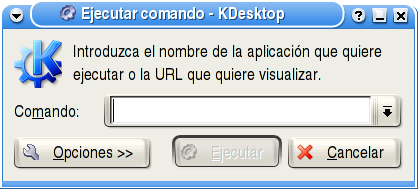
\includegraphics[width=0.45\textwidth]{imagenes/kde_lanzar.eps}
\label{kde_lanzar}}
\subfigure[Cuadro de diálogo avanzado {\tt EJECUTAR COMANDO}]{%
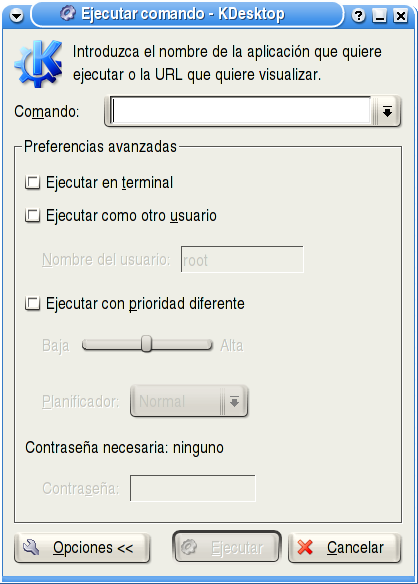
\includegraphics[width=0.45\textwidth]{imagenes/kde_lanzar_opt.eps}
\label{kde_lanzar_opt}}
\end{figure}

Igual que en el entorno de escritorio {\sf GNOME} en {\sf KDE} podemos
utilizar {\tt BLOQUEAR PANTALLA}  para proteger nuestro escritorio, si
tenemos que abandonarlo por cualquier  motivo, o {\tt TERMINAR SESIÓN}
para terminar nuestra sesión y volver al {\sf KDM} (Figura \ref{kdm}).
En este  sentido es importante  comentar que  una de las  opciones más
interesantes, disponible  a través del  {\tt MENÚ K}, es  {\tt INICIAR
NUEVA SESIÓN}. Gracias  a dicha opción podemos crear  una nueva sesión
de las  {\sf X}  y asociarla  a uno de  los terminales  virtuales (ver
página \pageref{terminal}). Esto nos permite  tener dos o más sesiones
abiertas en las {\sf X} y conmutar entre unas y otras.

Ya hemos  comentado que  el panel  de {\sf KDE}  puede contener  uno o
varios  botones de  aplicación, entre  otros elementos.  Habitualmente
entre esos  botones está  el acceso  al emulador  de terminal  de {\sf
KDE}, más conocido como {\sf Konsole}. Dicho botón suele ser el que se
simboliza como un  monitor (o terminal) con una  pequeña concha (shell
en inglés) en  una de sus esquinas. No debemos  confundirlo con el que
se  encuentra  por defecto  inmediatamente  a  su derecha  en  algunas
configuraciones de {\sf  KDE}, con unas barras de  colores pintadas en
el interior de un monitor. Este es el que abre el centro de control de
{\sf KDE},  mediante el  cual podemos configurar  la totalidad  de los
parámetros gráficos, estéticos, de  sonido, de rendimiento, de manejo,
etc.

Respecto a  las funciones de  los botones del  ratón en {\sf  KDE}, el
botón derecho sobre  el escritorio nos muestra un menú  con unas pocas
opciones, como  crear nuevos elementos en  nuestro escritorio (accesos
directos o enlaces, directorios, etc), ejecutar comandos, o configurar
el  escritorio. Si  pulsamos con  el botón  derecho del  nuestro ratón
sobre alguno de  los elementos del panel, veremos el  menú de contexto
asociado  al elemento.  Los menús  de contexto  de los  applets suelen
disponer  de  opciones  acorde  con  las  funciones  asignadas  a  los
mismos. Sin  embargo, las opciones  de los otros elementos  suelen ser
bastante estándar. Por  ejemplo, para mover el elemento  por el panel,
eliminarlo, cambiar sus  propiedades y acceder a  la configuración del
panel.  Concretamente esta  última opción  se denomina  {\tt MENÚ  DEL
PANEL}.

Los diferentes  elementos del  panel suelen  venir delimitados  por un
separador con un pequeña flecha negra.  Tanto si pulsamos con el botón
derecho del  ratón sobre dichos  separadores, como si pulsamos  con el
izquierdo sobre la flecha dispondremos de un menú similar al que hemos
comentado en el párrafo anterior (Figura \ref{kde_menu_panel}).

\begin{figura}{kde_menu_panel}{0.86}
\caption{Menú del panel de {\sf KDE}}
\label{kde_menu_panel}
\end{figura}


\subsection{Administración de archivos}

Uno de  los puntos fuertes  a favor de {\sf  KDE} es el  programa {\sf
Konqueror}\index{KDE!Konqueror}. {\sf  Konqueror} integra en  una sola
aplicación las funciones de administración de archivos, navegación web
y visor  de documentos.  Además de  todo eso se  trata de  un programa
completamente  ampliable  que  puede aumentar  sus  funcionalidades  a
partir  del uso  de {\em  plugins}. Gracias  a ellos  podemos realizar
tareas como  administrar los  archivos en los  equipos de  nuestra red
de  área local  (LAN),  administrar y  configurar  nuestro sistema  de
impresión, examinar nuestros CDs de audio, etc.

Cuando  pulsamos sobre  los  directorios o  dispositivos presentes  en
nuestro escritorio se nos abre {\sf  Konqueror} con el objetivo de que
podamos ver su contenido. En la Figura \ref{kde_konqueror_dir} podemos
ver  una  ventana  de  {\sf  Konqueror} donde  se  puede  explorar  el
directorio {\tt /etc}.

\begin{figura}{kde_konqueror_dir}{0.7}
\caption{Konqueror como administrador de archivos}
\label{kde_konqueror_dir}
\end{figura}

Como podemos apreciar la ventana de {\sf Konqueror} como administrador
de  archivos  es   similar  a  la  de   muchos  otros  administradores
de  archivos  que  hayamos  podido   ver.  La  mayor  parte  de  dicha
ventana  está ocupada  por los  iconos de  los directorios  y archivos
presentes en  el directorio  actual. Inmediatamente encima  tenemos la
{\em  barra  de  herramientas  de dirección}  donde  podemos  escribir
la  ruta  del  directorio  que  deseamos  explorar.  Puesto  que  {\sf
Konqueror}  es  un  programa  que integra  múltiples  funcionales,  en
dicha  barra  podemos  poner  la ruta  de  otros  recursos  diferentes
a  un   directorio.  Por  ejemplo,   podemos  poner  una   ruta  hacia
una  página  web   ({\tt  http://nombre\_equipo/ruta\_página}),  a  un
directorio  en  un   FTP  (ftp://nombre\_equipo/nombre\_directorio)  e
incluso  a  una  carpeta   compartida  de  Microsoft®  Windows®  ({\tt
smb://nombre\_netbios/carpeta}).

Como ya hemos comentado {\sf  Konqueror} dispone de características de
visor. Eso  significa que  pulsando sobre los  iconos de  los archivos
podemos ver su  contenido. En los supuestos en que  {\sf Konqueror} no
esté capacitado para  la visualización de un  determinado contenido se
abre  el programa  adecuado. De  la  misma manera  pulsando sobre  los
directorios  podemos navegar  por el  sistema de  ficheros de  nuestro
equipo. En la barra de herramientas de la parte superior disponemos de
botones para  subir un  nivel en  el árbol  de directorios,  avanzar o
retroceder, o  cambiar el modo de  vista de los archivos.  Usando {\em
arrastrar y soltar} podemos mover, copiar o crear un enlace a archivos
y directorios. Mientras  que pulsando con el  botón derecho disponemos
de  un  menú  de  contexto  con  algunas  opciones  adicionales,  como
renombrar,  eliminar,  o  editar  las  propiedades  de  un  archivo  o
directorio dado.

En el  lado de  la izquierda de  la ventana contamos  con el  panel de
navegación,  que  puede  desarrollar  diferentes  funciones  según  la
pestaña de la izquierda que  hayamos seleccionado. Podemos navegar por
nuestros marcadores, por  el historial de navegación, por  la Red, por
el  árbol de  directorios  de  nuestro equipo,  etc.  En general  {\sf
Konqueror} es  un programa  muy potente con  decenas de  funciones que
debemos probar.

Para  utilizar {\sf  Konqueror} como  navegador debemos  pulsar en  el
botón con un  globo terráqueo y un engranaje situado  en nuestro panel
(ver  Figura \ref{kde_panel}).  En  la Figura  \ref{kde_konqueror_web}
podemos ver el ejemplo de un ventana de {\sf Konqueror} con una pagina
web cargada.  La forma  de manejo del  mismo no dista  de la  forma de
manejo de cualquier otro navegador que hayamos utilizado.

\begin{figura}{kde_konqueror_web}{0.7}
\caption{Konqueror como navegador web}
\label{kde_konqueror_web}
\end{figura}


\subsection{Configuración del escritorio}

La  configuración para  personalizar el  escritorio se  puede realizar
desde el {\sf Centro  de control}\index{KDE!Centro de control} (Figura
\ref{kde_control}). Para  acceder al mismo basta  con seleccionar {\tt
PREFERENCIAS $\rightarrow$ CENTRO DE CONTROL} en el menú del entorno.

\begin{figura}{kde_control}{0.7}
\caption{Centro de control de {\sf KDE}}
\label{kde_control}
\end{figura}

En la parte derecha de la  ventana contamos con un árbol de categorías
en las que se clasifican  las diferentes opciones de configuración del
entorno de  escritorio {\sf KDE}.  Cuando seleccionamos una  de dichas
categorías  el  lado izquierdo  cambia  para  mostrarnos las  opciones
disponibles.

Cualquier  cambio  en la  configuración  debe  ser validado  con  {\tt
APLICAR}  para  que  tenga  efecto.  Adicionalmente  podemos  utilizar
{\tt  RESTAURAR} para  cancelar  las modificaciones  realizadas en  la
configuración, o {\tt PREDETERMINADO} para cargar la configuración por
defecto de {\sf KDE} en la categoría seleccionada. En caso de realizar
modificaciones  en  la  configuración  de  una  categoría,  y  de  que
intentemos cambiar  a otra sin  validar los  cambios de la  actual, el
sistema  nos avisará  de  la  situación y  nos  permitirá aplicar  los
cambios, deshacerlos, o cancelar el cambio de categoría.

Con todo esto, el amigo lector ya tiene opciones gráficas para elegir.
¡Que lo disfrute!.

